% ============================================================================
%  Common-Cause Failure Modelling in the Unified PDAG Framework
% ============================================================================
%  This file is manuscript-dissertation/5_refinements/ccf.tex and is \chapter{}-level.
% ----------------------------------------------------------------------------
\chapter{Integrating Common-Cause Failures into the Unified PDAG}
\label{chap:ccf_in_pdag}

\noindent\textbf{Scope.}\;Section~\ref{sec:unified_pra_dag} introduced the
probabilistic directed acyclic graph (PDAG) that unifies event-tree and
fault-tree logic.  The present chapter explains how \emph{common-cause
failures} (CCFs) are embedded into that same graph without altering the
execution, layering, or sampling mechanisms described in
Chapter~\ref{chap:mc_solver}.  The discussion complements the statistical CCF
models surveyed in Section~2.3 (\emph{Common-Cause Failures}) by detailing
(i)~how a \textit{CCF group} is mapped to PDAG nodes and edges, and
(ii)~why no additional variance-reduction or correlation-handling is required
inside the Monte-Carlo kernels.

% ----------------------------------------------------------------------------
\section{CCF Groups and Their Place in the PDAG}
\label{sec:ccf_group_def}

A \emph{CCF group} (CCFG) is a non-empty set
\(\mathcal{C}=\{c_1,c_2,\dots ,c_m\}\subseteq \mathcal{B}\) of basic events
that share at least one latent cause of failure.  The defining property is the
existence of a random variable
\(\Xi\) such that
\[\Pr[ X_{c_i}=1 \mid \Xi ] \text{ is identical } \forall i.\]
Three structural requirements ensure compatibility with the PDAG:
\begin{enumerate}
  \item No two CCFGs overlap: \(\mathcal{C}_i\cap\mathcal{C}_j=\varnothing\) for
        \(i\ne j\).  Overlaps are merged before analysis.
  \item Every basic event belongs to \emph{at most} one CCFG; components that
        are demonstrably independent stay outside any CCF modelling.
  \item The PDAG remains acyclic after inserting the CCF structures (see
        Section~\ref{subsec:ccf_insertion}).
\end{enumerate}
CCFG membership is derived from design information (shared components, common
location), operating experience, or expert elicitation and is therefore an
\emph{input} to the compilation workflow.

% ----------------------------------------------------------------------------
\section{Parametric CCF Models – A Recapitulation}
\label{sec:ccf_models_recap}

Section~2.3 enumerated several statistical formalisms for quantifying common-
cause probabilities: the Basic-Parameter Model, Alpha-Factor Model, Multiple-
Greek-Letter Model, Binomial Failure-Rate Model, and the one-parameter
Beta-Factor simplification.  These models differ mainly in the \\emph{parameter
vector}
\(\boldsymbol{\theta}_{\!\mathcal{C}}\) they attach to a group
\(\mathcal{C}\) and in how that vector is estimated from data.

For present purposes, we require only the mapping
\[\boldsymbol{\theta}_{\!\mathcal{C} } \longrightarrow
  \bigl\{\Pr[\text{exactly }k\text{ failures}]\bigr\}_{k=1}^{m}
  \;=\; \{\pi_{\mathcal{C},k}\}_{k=1}^{m} ,\]
where \(\pi_{\mathcal{C},k}\) is the unconditional probability that \emph{any
specific} subset of size \(k\) in \(\mathcal{C}\) fails owing to the common
cause during the reference mission time.  Table~\ref{tab:ccf_model_mapping}
lists the closed-form mappings for the most widespread models.

\begin{table}[t]
  \centering
  \caption{Mapping of model parameters to multiplicity probabilities
           \(\pi_{\mathcal{C},k}\).  The symbol \(m=|\mathcal{C}|\) denotes
           the group size.}
  \label{tab:ccf_model_mapping}
  \begin{tabular}{l@{\qquad}l}
    \toprule
    Model & $\pi_{\mathcal{C},k}$\\
    \midrule
    Beta-Factor ($\beta$) & $\pi_{k}=\begin{cases}
        1-\beta & k=1\\[4pt]
        \beta & k=m\\[2pt]
        0 & \text{otherwise}
      \end{cases}$\\[8pt]
    Alpha-Factor ($\alpha_k$) & $\displaystyle
      \pi_{k}=\frac{\alpha_k}{\binom{m-1}{k-1}}$\\[10pt]
    Basic-Parameter ($Q_k$) & $\pi_{k}=\dfrac{Q_k}{\sum_{j=1}^{m} \binom{m-1}{j-1}Q_j}$\\[10pt]
    MGL $(\beta,\gamma,\dots)$ & \emph{see Section~2.3 for $m\le 4$ closed forms}\\[8pt]
    BFR $(\nu,p)$ & $\displaystyle
      \pi_{k}= \frac{\nu}{\lambda_{c}}\, \binom{m}{k} p^{k}(1-p)^{m-k}
      \quad (k<m), \; \pi_{m}=\frac{\lambda^{(i)}}{\lambda_{c}}$\\
    \bottomrule
  \end{tabular}
\end{table}

The remainder of the chapter is \emph{model-agnostic}: once the vector
\(\{\pi_{\mathcal{C},k}\}\) is known, the graph-construction steps are
identical.

% ----------------------------------------------------------------------------
\section{Embedding a CCF Group into the PDAG}
\label{subsec:ccf_insertion}

Let \(\mathcal{C}=\{c_1,\dots,c_m\}\) be a CCFG with multiplicity
probabilities \(\pi_{\mathcal{C},k}\).  The insertion algorithm introduces one
auxiliary \textbf{CCF-root node}\;\(G_{\!\mathcal{C}}\) and at most
\(m-1\) \textbf{CCF-shadow nodes}.  All new nodes are classified as
\emph{gate-type} in the PDAG (set \(\mathcal{G}\)), thereby preserving the
basic-event set \(\mathcal{B}\).

\subsection{Step~1: Replace independent leaves.}  Each original basic event
\(c_i\) is kept \emph{in situ} but its independent failure probability is
scaled to account only for the \emph{independent} portion of failure,
\(p^{(\!I\!)}_{c_i}= (1-\lambda_{\text{ccf}})\,p_{c_i}\), where
\(\lambda_{\text{ccf}}=\sum_{k\ge 2} \pi_{\mathcal{C},k}\).  This is equivalent
to conditioning on the latent variable \(\Xi=0\) (no common-cause shock).

\subsection{Step~2: Insert CCF-root gate.}  A new node \(G_{\!\mathcal{C}}\)
collects \emph{two} input classes:
\begin{itemize}
  \item an \textit{auxiliary shock variable} \(S_{\mathcal{C}}\) that fires with
        probability \(\lambda_{\text{ccf}}\); and
  \item the set of leaves \(c_1,\dots,c_m\) (independent parts).  The gate type
        is OR.
\end{itemize}
The logical meaning is
\[G_{\!\mathcal{C}} = S_{\mathcal{C}} \;\lor\; c_1 \lor \dots \lor c_m.
\]
If the group is embedded inside redundancy logic this construction ensures that
an induced common-cause shock can bypass otherwise protective diversity.

\subsection{Step~3: Modeling multiplicity.}  Some CCF models specify not only
whether \emph{any} failure occurs but also \emph{how many} components are
involved.  To reproduce multiplicity‐specific probabilities we attach
\(m-1\) mutually exclusive \textit{shadow gates}
\(\{ H^{(2)}_{\mathcal{C}},\dots,H^{(m)}_{\mathcal{C}} \}\) as children of
\(S_{\mathcal{C}}\).  Shadow gate \(H^{(k)}_{\mathcal{C}}\) triggers exactly
\(k\) of the components via an OR-of-ANDs structure:
\[H^{(k)}_{\mathcal{C}}= \bigvee_{\substack{\mathcal{K}\subseteq\mathcal{C}\\|
\mathcal{K}|=k}}
           \bigl(\bigwedge_{c\in\mathcal{K}} F_c\bigr),
\]
where each \(F_c\) is a Boolean indicator that component \(c\) is affected by
this particular shock realization.  The shadow gate is assigned probability
\(\pi_{\mathcal{C},k}\).  Because the shadow nodes feed into the same outputs
as the original \(c_i\) leaves, downstream logic remains unaltered.

\subsection{Step~4: Maintain acyclicity.}  All newly created edges originate
from \emph{fresh} nodes introduced in this step; no existing PDAG edge is
re-directed upstream.  Therefore the global acyclicity invariant is preserved
trivially.

\subsection{Resulting subgraph.}  Figure~\ref{fig:ccf_embedding} illustrates
the transformation for \(m=3\) under a Beta-Factor model.

\begin{figure}[t]
  \centering
  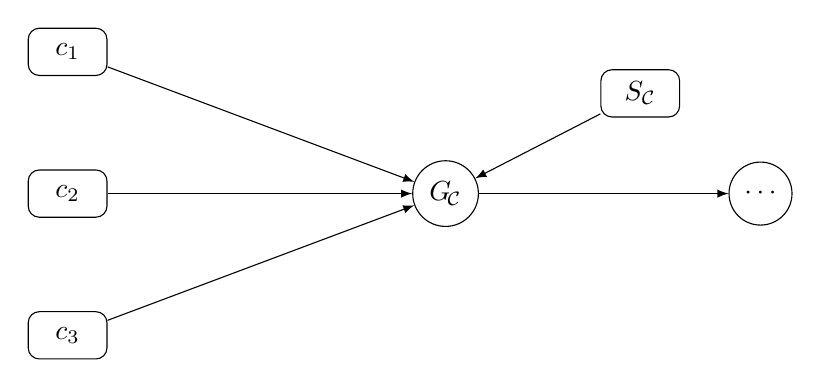
\begin{tikzpicture}[node distance=1.8cm,>=latex]
    \tikzstyle{basicevent}=[draw,rectangle,rounded corners,minimum width=1cm,minimum height=0.6cm]
    \tikzstyle{gate}=[draw,circle,minimum size=0.8cm]

    % Independent leaves
    \node[basicevent] (c1) {$c_1$};
    \node[basicevent,below of=c1] (c2) {$c_2$};
    \node[basicevent,below of=c2] (c3) {$c_3$};

    % CCF root
    \node[gate,right of=c2,xshift=3cm] (G) {$G_{\!\mathcal{C}}$};

    % Shock variable
    \node[basicevent,above right of=G,xshift=1.2cm] (S) {$S_{\mathcal{C}}$};

    % Edges
    \foreach \x in {c1,c2,c3}
        \draw[->] (\x) -- (G);
    \draw[->] (S) -- (G);

    % Output
    \node[gate,right of=G,xshift=2.2cm] (out) {$\cdots$};
    \draw[->] (G) -- (out);
  \end{tikzpicture}
  \caption{Embedding a three-component CCF group under the Beta-Factor model.
           The shock variable $S_{\mathcal{C}}$ fires with probability
           $\beta$ and forces simultaneous failure of $c_1,c_2,c_3$.  The
           independent portions $(1-\beta)p_{c_i}$ remain as separate leaves.
          }
  \label{fig:ccf_embedding}
\end{figure}

% ----------------------------------------------------------------------------
\section{Interplay with the Monte-Carlo Execution Model}
\label{sec:ccf_sampling}

The layered kernel strategy of Chapter~\ref{chap:mc_solver} assumes that each
leaf node is associated with an \emph{independent} random draw.  Introducing
$S_{\mathcal{C}}$ and the shadow nodes does not violate this assumption:
\begin{itemize}
  \item The augmented leaves \(\{S_{\mathcal{C}},c_1,\dots,c_m\}\) are   \emph{mutually independent}.  Correlation is introduced solely through the
        logical structure (shared downstream paths), not through coupled random
        numbers.  Therefore the existing bit-packed sampling kernel applies
        verbatim, drawing Bernoulli variates for \emph{each} auxiliary leaf.
  \item Any path in the PDAG traverses at most one of the mutually exclusive
        shadow nodes, ensuring that correlated failures are represented without
        double counting.
  \item Convergence diagnostics (Chapter~\ref{sec:convergence_criterion})
        operate on the empirical proportion of top-level node failures.  The
        presence of CCF nodes merely changes those proportions; the maths of
        Section~\ref{sec:convergence_criterion} is untouched.
\end{itemize}
Consequently, \textbf{no specialized sampling algorithm is required}; the
existing Monte-Carlo pipeline seamlessly handles CCFs once the PDAG has been
augmented as per Section~\ref{subsec:ccf_insertion}.

% ----------------------------------------------------------------------------
\section{Worked Example}
\label{sec:ccf_example}

Consider a two-pump parallel cooling loop where either pump suffices
(OR logic) but the pumps share a common lubrication system.  Let the independent
failure probabilities be \(p_A=3.0\times10^{-3}\) and \(p_B=3.0\times10^{-3}\),
with a Beta-Factor \(\beta=0.15\) for the common lubricant leak.

\paragraph{Mapping.}  The CCFG is \(\mathcal{C}=\{A,B\}\) (size $m=2$).  The
shock variable probability is $\lambda_{\text{ccf}}=\beta=0.15$; the
independent portions become $(1-\beta)p_A$ and $(1-\beta)p_B$.

\paragraph{PDAG augmentation.}  Following the procedure, we create nodes
$S_{\mathcal{C}}$ and $G_{\!\mathcal{C}}$; $G_{\!\mathcal{C}}$ feeds into the
existing OR-gate that models pump redundancy.  No other structural changes are
necessary.

\paragraph{Numerical impact.}  The top event ‘‘cooling loop fails’’ now has
probability
\[
  \Pr[\text{fail}] = \underbrace{\beta(1-(1-p_A)(1-p_B))}_{\text{CCF term}}
                      + \underbrace{(1-\beta)p_A p_B}_{\text{dual independent}}.
\]
Plugging the numbers yields
$\Pr[\text{fail}]=0.15\times 6\!\times10^{-3} + 0.85\times 9\!\times10^{-6}
  \approx 9.1\times10^{-4}$, which is dominated by the CCF term.

% ----------------------------------------------------------------------------
\section{Summary}

Common-cause failure groups are incorporated into the unified PDAG by
introducing auxiliary shock and shadow nodes whose probabilities encode any of
the established statistical models.  The transformation is purely structural
and preserves acyclicity, thereby allowing the existing layered Monte-Carlo
solver, convergence monitor, and data-parallel kernels to operate without
modification.  The approach thus unifies CCF treatment with the broader DAG-
based reliability analysis framework.

% ============================================================================

\section{Convergence Guarantees for CCF--Augmented Monte--Carlo Estimates}
\label{sec:ccf_convergence}

Let $Y^{(t)}$ be the indicator of a user--selected PDAG node ("event of
interest") during Monte--Carlo iteration $t\in\{1,\dots,T\}$.  The simulator
samples – 
independently across iterations – the failure state of every leaf, including
auxiliary CCF leaves $S_{\mathcal{C}}$ and the original basic events.  Define

\[\widehat{p}_T \;=\; \frac{1}{T}\sum_{t=1}^T Y^{(t)}
  \qquad\text{and}\qquad
  \sigma^2 = \operatorname{Var}[Y^{(1)}].\]

We prove that $\widehat{p}_T$ is an unbiased, strongly consistent estimator of
the true probability $p=\Pr[Y^{(1)}=1]$ and that it obeys the usual Central
Limit Theorem (CLT), irrespective of how many CCF groups the event intersects.

\subsection{Assumptions}
\label{subsec:ccf_conv_assumptions}
\begin{enumerate}
  \item \textbf{Iteration independence.}  All random variables associated with
        iteration $t$ are independent of those in iteration $t'\ne t$.  This is
        enforced by counter-based PRNGs whose counters differ in at least one
        component across iterations.
  \item \textbf{Finite variance.}  Because $Y^{(t)}\in\{0,1\}$, we have 
        $\sigma^2\le 1/4<\infty$.
  \item \textbf{CCF construction.}  Each CCF group is represented exactly as in
        Section~\ref{subsec:ccf_insertion}; in particular the auxiliary shock
        variable $S_{\mathcal{C}}$ is \emph{independent} of all other leaf
        variables.  Correlation among components is introduced solely through
        deterministic logic.
\end{enumerate}

\subsection{Unbiasedness and Strong Law of Large Numbers}
The event indicator in a single iteration is a measurable function of the leaf
sample vector
$\mathbf{X}^{(t)}=(X_b^{(t)})_{b\in\mathcal{B}\cup\{S_{\mathcal{C}}\}}$.
Given Assumption~1, $(Y^{(t)})_{t\ge1}$ is an independent and identically
distributed (i.i.d.) sequence with mean $\mathbb{E}[Y^{(1)}]=p$.
The Monte--Carlo estimator is therefore unbiased:
\[\mathbb{E}[\widehat{p}_T]=p\quad\forall T.\]
By Kolmogorov's Strong Law of Large Numbers applied to bounded i.i.d.
variables, we have almost sure convergence:
\[\widehat{p}_T \;\xrightarrow{\text{a.s.}}\; p\qquad (T\to\infty).\]

\subsection{Variance and CLT}
Because $Y^{(t)}$ are i.i.d.
with finite variance $\sigma^2$, the classical Central Limit Theorem yields
\[\sqrt{T}\,(\widehat{p}_T-p)
    \;\xrightarrow{\mathcal{D}}\; \mathcal{N}\bigl(0,\sigma^2\bigr).
\]
Hence the half--width of a $(1-\alpha)$ two–sided normal confidence interval is
\[h_T(z)=z\,\frac{\sigma}{\sqrt{T}},\qquad
  z=\Phi^{-1}(1-\alpha/2),\]
identical in form to Eq.~\eqref{eq:half_width}.  The presence of CCF logic can
at most change $\sigma^2$ (often it increases variance because failures become
more clustered) but \emph{does not} affect the $\mathcal{O}(1/\sqrt{T})$
convergence rate.

\subsection{Discussion of Dependence within Iterations}
Dependence between leaves \emph{within the same iteration} – introduced by
shared shock variables – is \emph{irrelevant} for the CLT because the theorem
operates on inter-iteration independence.  The proof therefore remains valid
under any Boolean post-processing of the leaves, including complex mixtures of
independent and common–cause failures.

\subsection{Conclusion}
Under the stated assumptions the Monte–Carlo estimator for any PDAG node,
whether or not it participates in common-cause groups, enjoys the same
unbiasedness, strong consistency, and $\mathcal{O}(1/\sqrt{T})$ confidence–
interval half–width as in the purely independent-failure case.  Consequently
the convergence diagnostics of Chapter~\ref{sec:convergence_criterion} apply
verbatim to CCF-augmented probabilities.
